\section{Notation and glossary}
\label{app:notation}

Table~\ref{tab:notation} consolidates the symbols used across the paper and the appendix.

\begin{table}[h]
\centering
\footnotesize
\setlength{\tabcolsep}{6pt}
\renewcommand{\arraystretch}{1.10}
\caption{Symbols, types, and where they are introduced.}
\label{tab:notation}
\begin{tabular}{@{}llp{0.55\linewidth}@{}}
\toprule
Symbol & Type / range & Meaning \\
\midrule
\multicolumn{3}{@{}l}{\textit{Network}}\\
$N$                                & $\mathbb{N}_{>0}$
                                   & Number of decoder layers in the released checkpoint. \\
$L_i$                              & $\mathbb{R}^{T\times d}\!\to\!\mathbb{R}^{T\times d}$
                                   & Pre-norm transformer block $i$, $0 \le i \le N-1$. \\
$f$                                & composition
                                   & Unmodified network: $f = L_{N-1} \circ \cdots \circ L_0$. \\
$T,d$                            & $\mathbb{N}_{>0}$
                                   & Sequence length and hidden dimension. \\
\addlinespace
\multicolumn{3}{@{}l}{\textit{Loop wrapper}}\\
$[a,b]$                            & $0 \le a \le b \le N-1$
                                   & Loop-window layer indices (contiguous). \\
$W$                                & $b-a+1$
                                   & Loop window width (in layers). \\
$K$                                & $\mathbb{N}_{\ge 1}$
                                   & Loop iteration count. \\
$g$                                & $\mathbb{R}^{T\times d}\!\to\!\mathbb{R}^{T\times d}$
                                   & Block operator: $g = L_b \circ \cdots \circ L_a$
                                     (Eq.~\ref{eq:block-op}). \\
$g^{(K)}$                          & $\mathbb{R}^{T\times d}\!\to\!\mathbb{R}^{T\times d}$
                                   & $K$-step iteration of $g$ under the chosen strategy
                                     (Section~\ref{sec:strategy}). \\
$\hat f(x)$                        & $\mathbb{R}^{T\times d}$
                                   & Looped network output \eqref{eq:wrapper}. \\
$g^{(K)}_{\mathrm{blk}},g^{(K)}_{\mathrm{lyr}}$
                                   & maps
                                   & Block-mode and layer-mode realizations of $g^{(K)}$
                                     \eqref{eq:block-mode}--\eqref{eq:layer-mode}. \\
\addlinespace
\multicolumn{3}{@{}l}{\textit{ODE view}}\\
$F_g$                              & $\mathbb{R}^{T\times d}\!\to\!\mathbb{R}^{T\times d}$
                                   & Window residual field $F_g(x) := g(x) - x$
                                     \eqref{eq:F}. \\
$F_{L_i}$                          & $\mathbb{R}^{T\times d}\!\to\!\mathbb{R}^{T\times d}$
                                   & Single-layer residual field $L_i(x) - x$. \\
$y_i(x)$                           & $\mathbb{R}^{T\times d}$
                                   & Intra-window residual stream at layer $i$
                                     \eqref{eq:block-effective-field}. \\
$h$                                & $\mathbb{R}_{>0}$
                                   & Forward-Euler step size; $h{=}1$ is the layer-built-in step. \\
$\alpha$                           & $(0,1]$
                                   & Damped-Euler coefficient $\alpha$; $\alpha = h$. \\
$\kappa_1,\ldots,\kappa_4$         & $\mathbb{R}^{T\times d}$
                                   & RK4 stage evaluations (Table~\ref{tab:strategies}). \\
$m,\beta$                        & $\mathbb{N},\,\mathbb{R}$
                                   & Anderson memory depth and mixing parameter. \\
\addlinespace
\multicolumn{3}{@{}l}{\textit{KV cache}}\\
$\mathcal{C}_i$                    & cache slot
                                   & Per-layer KV slot for layer $i$. \\
$\ell_i$                           & $\mathbb{N}$
                                   & Snapshot length of $\mathcal{C}_i$ before a loop iteration. \\
$c$                                & $\{\textsc{first},\textsc{last},\textsc{none}\}$
                                   & Cache strategy \eqref{eq:cache-strategy}. \\
\bottomrule
\end{tabular}
\end{table}

\section{Proofs}
\label{app:block-unroll}

\subsection{Proof of \texorpdfstring{\eqref{eq:block-effective-field}}{(9)}}

We expand block-mode iteration as an explicit chain of per-layer forward Euler steps and verify the closed-form identity stated in Section~\ref{sec:strategy}.

Let $g = L_b \circ L_{b-1} \circ \cdots \circ L_a$ be the loop window operator. Each constituent layer satisfies the single-layer forward Euler identity $L_i(z) = z + F_i(z)$. Fix an input $x$. Set $y_a(x) := x$ and define the \emph{intra-window residual stream} recursively by
\begin{equation}
y_{i+1}(x) \defeq L_i(y_i(x))
        \defeq y_i(x) + F_i\bigl(y_i(x)),
\qquad i = a, a+1, \ldots, b.
\label{eq:app-unroll-step}
\end{equation}
By construction, $g(x) = y_{b+1}(x)$. Summing \eqref{eq:app-unroll-step} from
$i = a$ to $i = b$ gives
\begin{equation*}
\sum_{i=a}^{b} (y_{i+1}(x) - y_i(x))
   = \sum_{i=a}^{b} F_i\bigl(y_i(x)).
\end{equation*}
The LHS telescopes to $y_{b+1}(x) - y_a(x) = g(x) - x$. Therefore
\begin{equation}
g(x) - x = \sum_{i=a}^{b} F_i(y_i(x)) \eqdef F_g(x),
\label{eq:app-block-effective-field}
\end{equation}
which is exactly \eqref{eq:block-effective-field}.

\subsection{Proof of \texorpdfstring{\eqref{eq:rk-beta-equivalence}}{(16)}}

By \eqref{eq:yi}, the standard $K$-substep forward Euler endpoint can be written as \[ F^{(K)}(x_0)=x_0+\frac{1}{K}\sum_{i=1}^{K}k_i. \] Substituting into the RHS of \eqref{eq:rk-beta-equivalence}, we have \begin{align*}
    \beta g(x_0)+(1-\beta)F^{(k)}(x_0)&=\beta g(x_0)+(1-\beta)x_0+\frac{1-\beta}{K}\sum_{i=1}^{K}k_i\\
    &=\beta g(x_0)+(1-\beta)x_0+\frac{1-\beta}{K}F_g(x_0)+\frac{1-\beta}{K}\sum_{i=2}^Kk_i\\
    &=x_0+\Par{\beta+\frac{1-\beta}{K}}k_1+\frac{1-\beta}{K}\sum_{i=2}^Kk_i,
\end{align*}
where the second and third lines use $k_1=F_g(x_0)=g(x_0)-x_0$. The conclusion follows upon expanding the LHS of \eqref{eq:rk-beta-equivalence} using the definitions in \eqref{eq:rk-beta-bi}.

\section{Decode loop algorithm}
\label{app:decode-loop}

The looped forward pass we patch into a frozen model has two regimes that share most code but differ in how the loop body interacts with the KV cache. During \emph{prefill} (\texttt{seq\_len > 1}, no past KV) the loop body is run with \texttt{use\_cache=False} and writes nothing to the cache; only a single \emph{stash pass} after the loop writes the canonical KV. During \emph{decode} (\texttt{seq\_len == 1}, an existing past KV) the loop body must attend to the past KV; otherwise, the new token is computed against a truncated context. However, it must also produce no net KV writes, since the stash pass will write the canonical entry afterwards. The mechanism is to snapshot per-loop-layer cache lengths before each loop iteration and crop back to those lengths immediately after.

\subsection{Decode-time looped forward pass}
\label{app:decode-algo-detailed}

Algorithm~\ref{alg:decode-loop-detailed} states the full block-mode decode-time forward pass as a single procedure, including the pre-loop / loop-body / stash / post-loop phases, the per-iteration snapshot/restore protocol, and the cache-strategy branch. Algorithm~\ref{alg:decode-loop-layer-detailed} states the layer-mode counterpart, which differs only in how iterations and snapshot/restore are nested.

\begin{figure}[t]
\centering
\begin{algorithm}[H]
\caption{Decode-time block-mode looped forward pass with KV cache}
\label{alg:decode-loop-detailed}
\begin{algorithmic}[1]
\Require new-token hidden state $x \in \mathbb{R}^{1 \times d}$, loop window $[a,b]$, loop count $K$, strategy update $\mathcal{S}$ (Euler/heavy-ball/Anderson/$\ldots$), cache strategy $c \in \{\textsc{first},\textsc{last},\textsc{none}\}$, per-layer KV cache $\mathcal{C} = (\mathcal{C}_0,\ldots,\mathcal{C}_{N-1})$
\Ensure Updated hidden state $x'$; $\mathcal{C}$ contains exactly one canonical KV entry per loop layer at the new decode position

\For{$i = 0,\ldots,a-1$} \Comment{pre-loop: standard layers, 1 KV each}
    \State $x \gets L_i(x;\mathcal{C}_i,\mathtt{use\_cache}=\textsc{T})$
\EndFor

\State $x_a \gets x$ \Comment{save pre-loop input for $c=\textsc{first}$}

\For{$i = a,\ldots,b$} \Comment{snapshot loop-layer cache lengths}
    \State $\ell_i \gets |\mathcal{C}_i|$
\EndFor

\For{$k = 1,\ldots,K$} \Comment{$K$ loop iterations under strategy $\mathcal{S}$}
    \State $y \gets x$ \Comment{evaluation starts from $x$}
    \For{$i = a,\ldots,b$} \Comment{run body with $\mathtt{use\_cache}=\textsc{T}$}
        \State $y \gets L_i(y;\mathcal{C}_i,\mathtt{use\_cache}=\textsc{T})$ \Comment{attn reads past KV at decode pos.}
    \EndFor
    \For{$i = a,\ldots,b$} \Comment{crop: discard iteration KV writes}
        \State $\mathcal{C}_i \gets \mathtt{crop}(\mathcal{C}_i,\ell_i)$ \Comment{net cache effect of body $=0$}
    \EndFor
    \State $x \gets \mathcal{S}(x,y,k)$ \Comment{e.g. $x+\alpha(y-x)$ for damped Euler}
\EndFor

\If{$c \neq \textsc{none}$} \Comment{stash phase: 1 KV write per loop layer}
    \State $z \gets \begin{cases}
        x, & c=\textsc{last},\\
        x_a, & c=\textsc{first}
    \end{cases}$
    \For{$i = a,\ldots,b$}
        \State $z \gets L_i(z;\mathcal{C}_i,\mathtt{use\_cache}=\textsc{T})$ \Comment{canonical KV at decode pos.}
    \EndFor
\EndIf

\For{$i = b+1,\ldots,N-1$} \Comment{post-loop: standard layers, 1 KV each}
    \State $x \gets L_i(x;\mathcal{C}_i,\mathtt{use\_cache}=\textsc{T})$
\EndFor

\State \Return $\textsc{LayerNorm}_{\text{out}}(x)$
\end{algorithmic}
\end{algorithm}
\end{figure}

\begin{figure}[t]
\centering
\begin{algorithm}[H]
\caption{Decode-time \emph{layer-mode} looped forward pass with KV cache (per-layer iteration; the safer default on MoE backbones, Section~\ref{sec:layer-mode}).}
\label{alg:decode-loop-layer-detailed}
\begin{algorithmic}[1]
\Require Same as Algorithm~\ref{alg:decode-loop-detailed}.
\Ensure Same as Algorithm~\ref{alg:decode-loop-detailed}.

\For{$i = 0, \ldots, a-1$} \Comment{pre-loop, standard}
    \State $x \gets L_i(x;\,\mathcal{C}_i,\,\mathtt{use\_cache}{=}\textsc{T})$
\EndFor

\State $x_a \gets x$

\For{$i = a, \ldots, b$} \Comment{outer: layers in order}
    \State $\ell_i \gets |\mathcal{C}_i|$ \Comment{snapshot length for layer $i$}
    \For{$k = 1, \ldots, K$} \Comment{inner: iterate this layer $K$ times}
        \State $y \gets L_i(x;\,\mathcal{C}_i,\,\mathtt{use\_cache}{=}\textsc{T})$
        \Comment{MoE: routing pinned across $k$}
        \State $\mathcal{C}_i \gets \mathtt{crop}(\mathcal{C}_i,\,\ell_i)$
        \Comment{discard iteration KV write}
        \State $x \gets \mathcal{S}(x,\,y,\,k)$
        \Comment{per-layer strategy update}
    \EndFor
    \State $z \gets x$ \textbf{if} $c{=}\textsc{last}$ \textbf{else} $x_a$
    \If{$c \neq \textsc{none}$}
        \State $z \gets L_i(z;\,\mathcal{C}_i,\,\mathtt{use\_cache}{=}\textsc{T})$
        \Comment{canonical KV at layer $i$}
    \EndIf
\EndFor

\For{$i = b+1, \ldots, N-1$} \Comment{post-loop, standard}
    \State $x \gets L_i(x;\,\mathcal{C}_i,\,\mathtt{use\_cache}{=}\textsc{T})$
\EndFor

\State \Return $\textsc{LayerNorm}_{\text{out}}(x)$
\end{algorithmic}
\end{algorithm}
\end{figure}

Lines 4--5 of Algorithm~\ref{alg:decode-loop-detailed} record the cache length each loop layer holds \emph{before} the body runs. The body in lines 6--12 is then executed $K$ times: each iteration runs the window with \texttt{use\_cache=True} (so attention reads the genuine past KV at the new decode position, line 9), and the immediately-following crop in lines 10--11 truncates the cache back to $\ell_i$, leaving zero net KV effect from the iteration. The strategy step on line 12 produces the next iterate $x$ from the current input $x$ and the body output $y$. Lines 13--16 are the stash phase: a single additional pass through the loop layers writes exactly one canonical KV entry per loop layer per decode position, using either the post-loop hidden state ($c{=}\textsc{last}$) or the pre-loop input ($c{=}\textsc{first}$) as the input to that pass. Lines 17--19 finish with the standard post-loop layers and the final output norm. The total cache delta of the entire procedure is exactly $b - a + 1$ entries regardless of $K$, which is identical to the unmodified model.

\subsection{Snapshot/restore}

\texttt{transformers.DynamicCache.update()} unconditionally appends the new $(k,v)$ to its per-layer tensor: there is no in-place overwrite mode. A naive $K$-iteration decode body would therefore write $K$ extra KV entries per loop layer at the same logical decode position, then attend to all of them on the next decode step, corrupting the cache and producing a sequence of phantom prefix tokens. The snapshot/restore pattern is the cheapest fix that (a) lets each loop iteration attend to the genuine past KV and (b) leaves the cache exactly as it was pre-iteration. The single canonical KV is then written by the stash pass on the chosen \texttt{cache\_strategy}. \texttt{layer-mode} looping uses an analogous per-layer snapshot/crop pair, applied $K$ times to one layer before moving on.

\subsection{\texttt{decode\_mode} variants}

We expose three \texttt{decode\_mode} settings. \texttt{bypass} skips the loop entirely on incremental decode and only loops during prefill (the default for loglikelihood-only evaluations). \texttt{full} loops every decode step. \texttt{first\_n} loops only on the first $n$ generated tokens (intended for CoT-prefix refinement; in practice never beats \texttt{full} when the loop helps and never recovers when it hurts). \texttt{full} is the default for the generation results reported in the main paper.

\section{Per-cell configurations}
\label{app:per-cell}

Table~\ref{tab:per-cell} lists every (model, benchmark) cell that is non-negative ($\Delta \geq -0.3$~pp) under the fixed recipe of Section~\ref{sec:setup}, i.e. $K{=}2$-stage Runge--Kutta at the depth-fraction window, block-mode for dense backbones and layer-mode for MoE, with \emph{no per-cell hyperparameter tuning}. Per-cell variations in absolute layer indices and in secondary settings (cache, decode) follow mechanically from each architecture's layer count; see Appendix~\ref{app:search-protocol} for the recipe specification. Each row gives the no-loop baseline, the best loop configuration found for that cell, and the resulting $\Delta$ in percentage points. Configurations are written as \texttt{[start--end] mode K strategy cache decode}, e.g.\ \texttt{[15--18] block K=3 Euler first full}.

\begin{table}[h]
\centering
\scriptsize
\setlength{\tabcolsep}{3pt}
\caption{Per-cell loop configurations across 7 model families under the out-of-the-box recipe of Section~\ref{sec:setup}. Mode = block / layer; cache $\in$ \{first, last, none\}; decode $\in$ \{bypass, full\}. The loop region iterates the indicated layer range $K$ times under the indicated strategy.}
\label{tab:per-cell}
\resizebox{\textwidth}{!}{%
\begin{tabular}{lllrrll}
\toprule
Model & Benchmark & Baseline & Loop & $\Delta$pp & Window / $K$ / strategy & cache / mode \\
\midrule
Qwen3-4B-Instruct  & MMLU-Pro 5sh CoT~[\citenum{wang2024mmlupro}]  & 57.14 & 59.79 & +2.64 & [15--18] $K{=}3$ Euler  & first / block / full \\
Qwen3-4B-Instruct  & GPQA-Main 0sh~[\citenum{rein2024gpqa}]     & 33.71 & 35.71 & +2.01 & [15--18] $K{=}3$ Euler  & first / block / full \\
Qwen3-4B-Instruct  & SciQ 0sh~[\citenum{welbl2017sciq}]          & 93.30 & 95.10 & +1.80 & [15--18] $K{=}3$ Euler  & first / block / full \\
Qwen3-4B-Instruct  & MMLU 0sh~[\citenum{hendrycks2021mmlu}]          & 68.15 & 69.45 & +1.30 & [15--18] $K{=}3$ Euler  & first / block / full \\
Qwen3-4B-Instruct  & CommonsenseQA 7sh~[\citenum{talmor2019csqa}] & 78.87 & 79.93 & +1.06 & [15--18] $K{=}3$ Euler  & first / block / full \\
Qwen3-4B-Instruct  & MedMCQA 0sh~[\citenum{pal2022medmcqa}]       & 53.40 & 54.13 & +0.73 & [11--14] $K{=}3$ Euler  & first / block / full \\
Qwen3-4B-Instruct  & ARC-Challenge 25sh~[\citenum{clark2018arc}]& 62.54 & 63.14 & +0.60 & [15--18] $K{=}3$ damped Euler $\alpha{=}0.5$ halt $\tau{=}0.05$ & first / block / full \\
Qwen3-4B-Instruct  & C-Eval 5sh~[\citenum{huang2023ceval}]        & 72.21 & 72.73 & +0.52 & [15--18] $K{=}3$ Euler  & first / block / full \\
Qwen3-4B-Instruct  & OpenBookQA 0sh~[\citenum{mihaylov2018obqa}]    & 40.20 & 40.60 & +0.40 & [11--14] $K{=}3$ Euler  & first / block / full \\
\midrule
Qwen3-4B-Base      & MMLU 5sh          & 73.27 & 73.61 & +0.34 & [15--18] $K{=}3$ Euler  & first / block / -- \\
Qwen3-4B-Base      & 16-task macro     & 63.98 & 65.03 & +1.05 & [15--18] $K{=}3$ Euler  & first / block / -- \\
Qwen3-1.7B-Base    & MMLU 5sh          & 62.68 & 63.01 & +0.34 & [12--15] $K{=}2$ damped Euler    & last  / block / -- \\
Qwen3-1.7B-Base    & 16-task macro     & 55.60 & 56.11 & +0.51 & [12--15] $K{=}2$ damped Euler    & last  / block / -- \\
Qwen3-0.6B-Base    & 16-task macro     & 47.87 & 48.43 & +0.56 & [12--15] $K{=}2$ heavy-ball $\alpha{=}0.5,\beta{=}0.5$ & last / layer / -- \\
\midrule
Llama-3.2-3B-Inst  & MMLU-Pro 5sh CoT  & --    & --    & +0.71 & [12--15] $K{=}2$ Euler  & first / block / full \\
Llama-3.2-3B-Inst  & GPQA-Main 0sh     & --    & --    & +0.67 & [12--15] $K{=}2$ Euler  & first / block / full \\
Llama-3.2-3B-Inst  & MMLU 5sh          & --    & --    & +0.72 & [16--19] $K{=}2$ Euler  & last  / layer / bypass \\
Llama-3.2-3B-Inst  & OpenBookQA 0sh    & --    & --    & +0.40 & [20--23] $K{=}3$ Euler  & last  / block / bypass \\
\midrule
Qwen1.5-MoE-A2.7B  & ARC-Challenge 25sh& 48.29 & 50.59 & +2.30 & [13--16] $K{=}3$ Euler  & first / block / full \\
Qwen1.5-MoE-A2.7B  & CommonsenseQA 7sh & 79.61 & 81.33 & +1.72 & [10--13] $K{=}2$ Euler  & first / block / full \\
Qwen1.5-MoE-A2.7B  & OpenBookQA 0sh    & 31.60 & 33.20 & +1.60 & [14--17] $K{=}3$ Euler  & first / block / full \\
Qwen1.5-MoE-A2.7B  & SciQ 0sh          & 94.80 & 95.10 & +0.30 & [14--17] $K{=}3$ Euler  & first / block / full \\
\midrule
DeepSeek-V2-Lite   & ARC-Challenge 25sh& 57.94 & 58.79 & +0.85 & [13--16] $K{=}2$ Euler  & first / layer / bypass \\
DeepSeek-V2-Lite   & OpenBookQA 0sh    & 35.80 & 36.60 & +0.80 & [13--16] $K{=}2$ Euler  & first / block / bypass \\
DeepSeek-V2-Lite   & MMLU (1500)       & --    & --    & +0.56 & [10--13] $K{=}3$ Euler  & first / block / bypass \\
DeepSeek-V2-Lite   & CommonsenseQA 7sh & 75.43 & 75.92 & +0.49 & [11--14] $K{=}2$ Euler  & first / block / bypass \\
\midrule
Moonlight-16B-A3B  & OpenBookQA 0sh    & --    & --    & +1.20 & [8--11]  $K{=}3$ Euler  & first / block / bypass \\
Moonlight-16B-A3B  & GPQA-Main 0sh     & --    & --    & +0.89 & [15--18] $K{=}2$ Euler  & first / layer / bypass \\
Moonlight-16B-A3B  & ARC-Challenge 25sh& --    & --    & +0.51 & [11--14] $K{=}2$ Euler  & first / layer / bypass \\
Moonlight-16B-A3B  & CommonsenseQA 7sh & --    & --    & +0.49 & [11--14] $K{=}2$ Euler  & first / layer / bypass \\
\midrule
Qwen3-30B-A3B-Inst & CommonsenseQA 7sh & 78.71 & 79.85 & +1.14 & [22--24] $K{=}2$ Euler  & first / block / bypass \\
\bottomrule
\end{tabular}%
}
\end{table}

We ablate strategy, $K$, window width, and cache strategy on Qwen3-1.7B-Base at canonical position [12-15]. Table~\ref{tab:ablations} reports the results.

\begin{table}[h]
\centering
\caption{Ablations of the loop wrapper on Qwen3-1.7B-Base \texttt{[12--15]}. $\Delta$pp on the $16$-task macro vs.\ the no-loop baseline; the within-family reference cell is damped Euler at $K{=}2,\,\alpha{=}0.5$. $\downarrow\downarrow$ marks catastrophic divergence (perplexity blowup or strict-format regression). Bold marks the per-axis best.}
\label{tab:ablations}
\small
\renewcommand{\arraystretch}{1.15}
\setlength{\tabcolsep}{5pt}
\resizebox{0.92\textwidth}{!}{%
\begin{tabular}{@{}l *{6}{c}@{}}
\toprule
\multicolumn{7}{@{}l}{\textbf{(a) Window width $n$} \,(centered on \texttt{[12--15]}, $K{=}2$ damped Euler)}\\
\midrule
$n$        & 1     & 3     & \textbf{4}        & 6     & 12    & 28 (full)             \\
\cmidrule(lr){2-7}
$\Delta$pp & +0.18 & +0.21 & \textbf{+0.55}    & -0.82 & -0.63 & $\downarrow\downarrow$  \\
\midrule
\multicolumn{7}{@{}l}{\textbf{(b) Iteration count $K$ \& strategy} \,($n{=}4$, mid-window)}\\
\midrule
           & \multicolumn{2}{c}{\textit{naive loop}}
           & \multicolumn{2}{c}{\textit{damped Euler}}
           & \multicolumn{2}{c}{\textit{higher-order \& accel.}} \\
\cmidrule(lr){2-3}\cmidrule(lr){4-5}\cmidrule(lr){6-7}
$K$        & $K{=}2$       & $K{=}4$
           & $K{=}2,\,\alpha{=}0.5$ & $K{=}3,\,\alpha{\approx}1/3$
           & \multicolumn{2}{c}{Anderson, RK4, Heun, $\ldots$} \\
\cmidrule(lr){2-3}\cmidrule(lr){4-5}\cmidrule(lr){6-7}
$\Delta$pp & +0.51       & -10.21$_{\text{(0.6B)}}$
           & \textbf{+0.55} & +1.05$_{\text{(4B)}}$
           & \multicolumn{2}{c}{see Table~\ref{tab:solver-ablation}} \\
\midrule
\multicolumn{7}{@{}l}{\textbf{(c) Cache strategy} \,($n{=}4$, $K{=}2$ damped Euler)}\\
\midrule
           & \multicolumn{3}{c}{\textit{16-task aggregate}}
           & \multicolumn{3}{c}{\textit{per-benchmark detail (\texttt{none} regression)}} \\
\cmidrule(lr){2-4}\cmidrule(lr){5-7}
strategy   & \texttt{first}    & \texttt{last}     & \texttt{none}
           & GSM8K~[\citenum{cobbe2021gsm8k}] \texttt{none} & MMLU-Pro~[\citenum{wang2024mmlupro}] \texttt{none} & MBPP~[\citenum{austin2021mbpp}] $\Delta_{\texttt{last-first}}$ \\
\cmidrule(lr){2-4}\cmidrule(lr){5-7}
$\Delta$pp & $\geq$\textbf{0} & $\geq$\textbf{0} & $\downarrow\downarrow$
           & -58.91          & -8.86           & +0.60              \\
\bottomrule
\end{tabular}%
}
\end{table}

Table~\ref{tab:solver-ablation} pulls representative rows from the $40+$ configuration sweep in Appendix~\ref{app:strategy-ablation}, demonstrating that higher-order integrators do not help. The looped block is not a smooth ODE, and Anderson-style fixed-point acceleration~\citep{walker2011anderson,bai2019deep,bai2020multiscale} overshoots because the block is not contractive enough. Within our strategy family, $K{=}2$-stage Runge--Kutta with $n{=}4$ and \texttt{cache=first} is the robust default.

\begin{table}[h]
\centering
\caption{Higher-order ODE solvers and fixed-point accelerators vs.\ damped Euler. Numbers are 16-task macro $\Delta$pp on Qwen3-1.7B-Base \texttt{[12--15]}; each column is referenced to its own damped Euler $K{=}2,\,\alpha{=}0.5$ baseline. ``---'' = not tested in that mode. The full sweep ($40+$ configurations across both modes) is reported in Appendix~\ref{app:strategy-ablation}.}
\label{tab:solver-ablation}
\small
\setlength{\tabcolsep}{8pt}
\renewcommand{\arraystretch}{1.12}
\begin{tabular*}{\textwidth}{@{\extracolsep{\fill}}llcc@{}}
\toprule
Family & Method ($K{=}2$ unless noted) & Block-mode $\Delta$ & Layer-mode $\Delta$ \\
\midrule
\textit{Reference}
   & damped Euler ($\alpha{=}0.5$, $h{=}1/2$)
   & 0.00 & 0.00 \\
\midrule
\multirow{3}{*}{\textit{Higher-order Runge--Kutta}}
   & midpoint (RK2) & -0.85 & -1.96 \\
   & Heun (RK2)     & -0.92 & -1.90 \\
   & RK4            & -0.65 & -2.34 \\
\midrule
\multirow{4}{*}{\textit{Fixed-point acceleration}}
   & heavy-ball ($\alpha{=}0.5,\,\beta{=}0.3$)
       & -0.12 & -0.06 \\
   & Anderson ($K{=}4,\,m{=}2,\,\beta{=}0.5$)
       & -0.96 & ---      \\
   & Aitken $\Delta^2$ (safeguarded)
       & -7.00 & ---      \\
   & Anderson, worst ($K{=}8,\,m{=}3,\,\beta{=}1.0$)
       & \textbf{-18.06} & \textbf{-19.56} \\
\bottomrule
\end{tabular*}
\end{table}

\subsection{Patterns visible in the per-cell table}

Three patterns generalize across families: (i) the winning window sits at depth fraction 0.4--0.7 for all dense and MoE models tested, with sub-1B models sometimes preferring a much earlier band (e.g.\ Llama-3.2-1B GPQA prefers \texttt{[4--7]} on a 16-layer model); (ii) MoE models systematically prefer \texttt{layer-mode} $K{=}2$ over \texttt{block-mode} $K{=}3$ on individual cells, consistent with expert-routing thrash hurting block-mode at $K \geq 3$; and (iii) \texttt{cache=first} dominates \texttt{cache=last} on long-prompt cells, while \texttt{cache=last} is mildly preferred for short structured generation (MBPP, +0.6 pp over \texttt{first}).

\section{Strategy ablation tables}
\label{app:strategy-ablation}

This section reproduces, in full numerical form, the strategy comparisons that motivate a main result of the paper: \emph{every classical fixed-point acceleration we tried fails to outperform $K{=}2$-stage Runge--Kutta (Algorithm~\ref{alg:rk_beta}) with $\beta{=}0.5$ on the looped block.} All entries use Qwen3-1.7B-Base on the canonical loop window \texttt{[12--15]} with block-mode looping. The reference is $K{=}2$ damped Euler at 0.56113 macro on the 16-task aggregate.

\subsection{Anderson, heavy-ball, Aitken, \texorpdfstring{$\alpha$}{alpha}-schedules}

\begin{table}[h]
\centering
\footnotesize
\caption{Fixed-point acceleration sweep (Qwen3-1.7B-Base, \texttt{[12--15]}, block-mode). $\Delta$ is in percentage points vs the $K{=}2$ damped Euler reference 56.113. Sorted best$\to$worst.}
\label{tab:phase6}
\begin{tabular}{lclcc}
\toprule
Strategy & $K$ & Hyperparameters & 16-task & $\Delta$ vs $K{=}2$ damped Euler \\
\midrule
Euler-sched     & 2 & $\alpha{=}[0.6,0.4]$       & 56.085 & -0.028 \\
heavy-ball      & 2 & $\alpha{=}0.5,\beta{=}0.3$ & 55.999 & -0.115 \\
heavy-ball      & 2 & $\alpha{=}0.5,\beta{=}0.5$ & 55.993 & -0.120 \\
heavy-ball      & 2 & $\alpha{=}0.7,\beta{=}0.3$ & 55.946 & -0.167 \\
heavy-ball      & 4 & $\alpha{=}0.3,\beta{=}0.5$ & 55.927 & -0.186 \\
Euler-sched     & 4 & $\alpha{=}[0.7,0.5,0.3,0.1]$ & 55.478 & -0.636 \\
Euler-sched     & 3 & $\alpha{=}[0.7,0.5,0.3]$    & 55.252 & -0.861 \\
Anderson        & 4 & $m{=}2,\beta{=}0.5$        & 55.153 & -0.960 \\
Euler-sched     & 3 & $\alpha{=}[0.3,0.5,0.7]$    & 55.036 & -1.077 \\
Anderson        & 6 & $m{=}3,\beta{=}0.5$        & 54.722 & -1.391 \\
Anderson        & 3 & $m{=}2,\beta{=}1.0$        & 54.373 & -1.740 \\
Anderson        & 6 & $m{=}2,\beta{=}0.5$        & 54.333 & -1.781 \\
heavy-ball      & 4 & $\alpha{=}0.5,\beta{=}0.3$ & 54.044 & -2.069 \\
Euler-sched     & 4 & $\alpha{=}[0.4,0.6,0.6,0.4]$& 54.005 & -2.108 \\
heavy-ball      & 4 & $\alpha{=}0.5,\beta{=}0.5$ & 53.495 & -2.618 \\
Anderson        & 4 & $m{=}3,\beta{=}1.0$        & 52.655 & -3.458 \\
heavy-ball      & 4 & $\alpha{=}0.5,\beta{=}0.7$ & 52.562 & -3.552 \\
Anderson        & 4 & $m{=}2,\beta{=}1.0$        & 52.032 & -4.082 \\
heavy-ball      & 3 & $\alpha{=}1.0,\beta{=}0.5$ & 51.236 & -4.877 \\
Aitken $\Delta^2$ & 2 & safeguarded             & 49.109 & -7.004 \\
Aitken $\Delta^2$ & 4 & safeguarded             & 48.318 & -7.795 \\
Aitken $\Delta^2$ & 6 & safeguarded             & 44.921 & -11.192 \\
Anderson        & 6 & $m{=}2,\beta{=}1.0$        & 44.261 & -11.852 \\
Anderson        & 8 & $m{=}3,\beta{=}1.0$        & 38.058 & -18.056 \\
\bottomrule
\end{tabular}
\end{table}

24 configurations; \emph{none} beat $K{=}2$ damped Euler. The closest is the $[0.6,0.4]$ damped-Euler schedule at -0.03 pp (statistical tie). Anderson extrapolation degrades smoothly with $K$ and catastrophically at $K{=}8$ (-18 pp), confirming the residual sequence $x_{k+1} - x_k$ in the loop is not approaching zero in a way Anderson can exploit.

\subsection{Norm stabilization and polynomial blending}

\begin{table}[h]
\centering
\footnotesize
\caption{Norm-stab and poly-blend sweep, same setup. $\Delta$
in pp vs $K{=}2$ damped Euler reference; baseline (no loop) sits at $55.598$.}
\label{tab:phase7}
\begin{tabular}{lrlrr}
\toprule
Strategy & $K$ & Hyperparameters & 16-task & $\Delta$ vs $K{=}2$ damped Euler \\
\midrule
norm\_stab  & 2 & $\alpha{=}0.5$               & 56.059 & -0.055 \\
poly\_blend & 2 & $w{=}[0.4,0.2,0.4]$          & 55.974 & -0.139 \\
poly\_blend & 2 & $w{=}[0.1,0.4,0.5]$          & 55.884 & -0.229 \\
poly\_blend & 2 & $w{=}[0.2,0.3,0.5]$          & 55.753 & -0.360 \\
poly\_blend & 2 & $w{=}[0.0,0.5,0.5]$          & 55.599 & -0.514 \\
poly\_blend & 2 & $w{=}[0.25,0.25,0.5]$        & 55.371 & -0.742 \\
poly\_blend & 2 & $w{=}[0.5,0.0,0.5]$          & 55.107 & -1.006 \\
norm\_stab  & 2 & $\alpha{=}0.7$               & 55.009 & -1.105 \\
poly\_blend & 3 & $w{=}[0.2,0.2,0.2,0.4]$      & 54.818 & -1.295 \\
poly\_blend & 3 & $w{=}[0.1,0.2,0.3,0.4]$      & 54.681 & -1.433 \\
norm\_stab  & 3 & $\alpha{=}0.5$               & 53.270 & -2.844 \\
norm\_stab  & 2 & $\alpha{=}1.0$               & 52.302 & -3.811 \\
norm\_stab  & 6 & $\alpha{=}0.3$               & 49.560 & -6.554 \\
norm\_stab  & 3 & $\alpha{=}0.7$               & 49.338 & -6.776 \\
norm\_stab  & 4 & $\alpha{=}0.5$               & 49.067 & -7.046 \\
norm\_stab  & 3 & $\alpha{=}1.0$               & 43.101 & -13.013 \\
\bottomrule
\end{tabular}
\end{table}

16 additional configurations; again none beat $K{=}2$ damped Euler. \texttt{norm\_stab} (rescaling each iterate to a fixed L2 norm) is catastrophic at $K \geq 3$, confirming that the iterates are diverging \emph{in direction} too.

\subsection{Layer-mode replicates the result}

In layer-mode the loop body is $L_i^K$ applied per-layer rather than $g^K = (L_b \circ \cdots \circ L_a)^K$ applied to the block. Reference: layer-mode $K{=}2$ damped Euler at 56.347 on the same window.

\begin{table}[h]
\centering
\footnotesize
\caption{Layer-mode strategy sweep on Qwen3-1.7B-Base \texttt{[12--15]}. $\Delta$ vs layer-mode $K{=}2$ damped Euler.}
\label{tab:phase18}
\begin{tabular}{lrr}
\toprule
Recipe & 16-task & $\Delta$ vs layer $K{=}2$ damped Euler \\
\midrule
$K{=}2$ heavy-ball $\alpha{=}0.5,\beta{=}0.3$ & 56.292 & -0.056 \\
$K{=}2$ poly\_blend $w{=}[0.25,0.5,0.25]$    & 56.181 & -0.167 \\
$K{=}3$ damped Euler $\alpha{=}0.3$           & 55.278 & -1.069 \\
$K{=}4$ Euler                                 & 55.240 & -1.107 \\
$K{=}2$ damped Euler $\alpha{=}0.7$           & 55.196 & -1.151 \\
$K{=}6$ Euler                                 & 54.998 & -1.350 \\
$K{=}2$ Heun                                  & 54.445 & -1.902 \\
$K{=}2$ midpoint                              & 54.385 & -1.962 \\
$K{=}1$ RK4                                   & 54.242 & -2.105 \\
$K{=}1$ midpoint                              & 54.178 & -2.169 \\
$K{=}2$ norm\_stab $\alpha{=}0.5$             & 54.098 & -2.249 \\
$K{=}1$ Heun                                  & 54.060 & -2.287 \\
$K{=}2$ RK4                                   & 54.005 & -2.342 \\
$K{=}3$ heavy-ball $\alpha{=}0.5,\beta{=}0.3$ & 51.830 & -4.517 \\
$K{=}3$ Anderson $m{=}2,\beta{=}1.0$          & 44.035 & -12.312 \\
$K{=}4$ Anderson $m{=}2,\beta{=}1.0$          & 36.785 & -19.562 \\
\bottomrule
\end{tabular}
\end{table}

Higher-order ODE solvers (Heun, midpoint, RK4) degrade more dramatically in layer-mode (-1.7 to -2.3 pp) than in block-mode (-0.7 to -1.1 pp): per-layer the map $L_i$ is \emph{not} better conditioned for higher-order integration than the composed $g$. Anderson in layer-mode is even more severe (-19.6 pp at $K{=}4$). The combined sweep covers 40+ acceleration configurations, and \emph{none} robustly beats Runge--Kutta. This is the empirical basis for the claim that \emph{the looped transformer block is not a contractive map}, so fixed-point acceleration is the wrong tool.

\section{Compute and reproducibility}
\label{app:reproducibility}

\subsection{Software stack}

All evaluations use \texttt{lm-evaluation-harness} v0.4.11 with deterministic seeds, default sampling settings per task, and \texttt{transformers} 4.46. Looped forwards are implemented as monkey patches on the model's \texttt{Model} class; patching preserves all original generation/eval code paths and is reversible. For the DeepSeek-V2/V3 family we additionally ship a small \texttt{DynamicCache} compatibility shim that re-exposes \texttt{seen\_tokens}/\texttt{get\_max\_length}/\texttt{get\_usable\_length} to the bundled \texttt{modeling\_deepseek} remote code.

\subsection{Per-model resource footprint}

\begin{table}[h]
\centering
\footnotesize
\caption{Approximate single-GPU memory and per-job wallclock for the representative jobs. Times are for the full 16-task suite at default \texttt{lm-eval-harness} batch sizes; CoT generation jobs (e.g.\ MMLU-Pro 5sh CoT) take 2--5$\times$ longer in \texttt{decode\_mode=full}.}
\begin{tabular}{lrll}
\toprule
Model & VRAM (bf16) & Hardware used & Eval-suite wallclock \\
\midrule
Qwen3-0.6B-Base / -Instruct       &  $\sim$2~GB & A100-40 / H100-80 & $\sim$1~h \\
Qwen3-1.7B-Base                   &  $\sim$4~GB & A100-40 / H100-80 & $\sim$2~h \\
Qwen3-4B-Base / -Instruct         &  $\sim$8~GB & A100-40 / H100-80 & $\sim$3~h \\
Llama-3.2-1B / -3B-Instruct       &  $\sim$3--7~GB & A100-40 / H100-80 & $\sim$2~h \\
Qwen1.5-MoE-A2.7B-Chat            &  $\sim$30~GB & H100-80 & $\sim$4~h \\
DeepSeek-V2-Lite-Chat (16B/2.4B)  &  $\sim$32~GB & H100-80 & $\sim$5~h \\
Moonlight-16B-A3B-Instruct        &  $\sim$32~GB & H100-80 & $\sim$8~h (\texttt{decode=full} 21~h) \\
Qwen3-30B-A3B-Instruct            &  $\sim$60~GB & H100-80 & $\sim$10~h (19-task 0-shot) \\
\bottomrule
\end{tabular}
\end{table}


\section{Failed configurations log}
\label{app:failures}

This section documents the configurations we tried that broke. We include them in the appendix so future work knows what does \emph{not} work, and so the main claims are read against an honest log of what \emph{was} tried.

\subsection{Catastrophic collapse on naive \texorpdfstring{$K{=}4$}{K=4} looping}

The first ablation we ran (Qwen3-0.6B-Instruct, 6-task) tested naive $K{=}4$ looping ($x \leftarrow g(x)$ four times, no damping). This resulted in lambada perplexity blowing up from $\sim$13 to \textbf{1054.12}, and 16-task macro dropped -10.21 pp. This is the original empirical observation that the block is not a contraction: undamped iteration diverges visibly within four applications, even on a window of just four mid layers.

\subsection{\texttt{cache=none} is uniformly catastrophic on decode}

Setting \texttt{cache\_strategy="none"} (no KV is written for the loop region; the next decode token must attend through it as if those layers contributed no past) collapses generation benchmarks. As an example, on Qwen3-4B-Instruct with \texttt{[15--18]} $K{=}3$:

\begin{itemize}
\item MBPP 3-shot~\citep{austin2021mbpp}: pass@1 38.20 vs 61.60 ($-23.40$~pp).
\item MMLU-Pro 5-shot~\citep{wang2024mmlupro}: 48.29 vs 57.14 ($-8.86$~pp).
\end{itemize}

The takeaway is that the loop region must contribute \emph{some} KV to the cache for autoregressive decode. \texttt{cache=first} (pre-loop hidden state) and \texttt{cache=last} (post-loop hidden state) both work; \texttt{first} dominates for long CoT and \texttt{last} for short structured output.

\subsection{Wide loop windows blow up}

On Qwen3-1.7B-Base \texttt{[12--15]}, $n{=}4$ is the canonical setting. Widening the window degrades performance monotonically:
\begin{itemize}
\item $n{=}6$, \texttt{[11..16]}: -0.82 pp on 16-task macro, lambada PPL drifts up.
\item $n{=}12$, \texttt{[8..19]}: -0.63 pp; the loop now spans nearly the entire ``representational middle'' of the network.
\item $n{=}28$ (whole network): lambada PPL blows up to $\mathbf{6.3 \times 10^5}$, total collapse.
\end{itemize}
In particular, applying the entire model twice is not a meaningful operation under training-free patching. The contracting region is a contiguous mid-band of about 4 layers, and applying a non-contracting region $K$ times amplifies its non-contraction.

\subsection{Higher-order ODE solvers all degrade}

In both block-mode and layer-mode, Heun, midpoint, and RK4 lose to damped Euler. Block-mode losses are -0.7 to -1.1 pp; layer-mode losses are -1.7 to -2.3 pp. Higher-order methods assume the underlying vector field is smooth and the iteration is approximating an ODE flow; the looped block does not satisfy this in practice.

\subsection{Position-search overfits to the 16-task aggregate}

Two independent windows beat canonical \texttt{[12--15]} by +0.9 to +1.3 pp on the 16-task aggregate but \emph{regressed} -1.0 to -1.4 pp on held-out MMLU 5-shot~\citep{hendrycks2021mmlu}:
\begin{itemize}
\item Qwen3-0.6B-Base \texttt{[8--11]}: +1.33 16-task, -1.21 MMLU 5sh.
\item Qwen3-1.7B-Base \texttt{[7--10]}: +0.92 16-task, -1.38 MMLU 5sh.
\end{itemize}
The 16-task suite is not a robust target for sub-1pp claims; small per-task MMLU subjects (100--300 examples) drive false signal. We kept the suite as a \emph{screen} for promising configurations and re-validated every ``win'' on MMLU 5-shot ($\sim$14k examples) before reporting.

\subsection{Layer-mode \texorpdfstring{$K{=}3$}{K=3} is uniformly catastrophic}

In layer-mode, $K{=}3$ heavy-ball on Qwen3-4B-Base \texttt{[15--18]} loses -5.0 pp on 16-task and -6.0 pp on MMLU 5-shot vs canonical ($K{=}3$ Euler block-mode). Layer-mode tolerates only mild $K{=}2$ Runge--Kutta; iterating individual layers more than twice produces strongly out-of-distribution per-layer states.

\subsection{Anderson at \texorpdfstring{$K{=}8$}{K=8}}

For completeness, Anderson $m{=}3,\beta{=}1.0,K{=}8$ on Qwen3-1.7B-Base \texttt{[12--15]} drops 16-task macro by \textbf{-18.06} pp. This is the strongest evidence that the block is not contractive: a method that is provably optimal on contractive maps (Anderson with $m \geq 1$) is the worst single configuration we found.

\subsection{Sub-1B knowledge MC}

We isolate a small set of cells unflipped after per-cell tuning, all on Llama-3.2-1B knowledge MC: MMLU~\citep{hendrycks2021mmlu} (-0.63) and MMLU-Pro~\citep{wang2024mmlupro} (-1.36). Sub-scale models below $\sim$1.7B for Qwen3 and $\sim$3B for Llama lack the mid-layer redundancy the loop relies on. Notably, GPQA-Main~\citep{rein2024gpqa} \emph{does} flip positive on the same Llama-3.2-1B checkpoint (+1.79) at the very-early window \texttt{[4--7]}, so the boundary is task-dependent rather than absolute.

\section{Concentration of benchmark gains}
\label{app:per-subject}

Across MMLU's~\citep{hendrycks2021mmlu} 57 subjects, MMLU-Pro's~\citep{wang2024mmlupro} 14 categories, and MMLU-Redux's 30 subjects, the loop wrapper produces a non-uniform improvement profile: gains concentrate on STEM and quantitative-reasoning subjects where the baseline is furthest from ceiling. Tables~\ref{tab:mmlu-base-subjects} and~\ref{tab:mmlu-redux-subjects} list the $\geq$+2 pp subjects on the two clearest cases.

\begin{table}[h]
\centering
\footnotesize
\caption{MMLU 5-shot per-subject deltas on Qwen3-4B-Base under \texttt{[17--19]} $K{=}2$ Euler. The 57-subject macro is essentially tied at this configuration (73.01$\to$72.90, -0.11 pp), but the \emph{distribution} of gains is highly non-uniform: seven subjects gain $\geq$+2 pp, all on hard STEM/quantitative content, while small offsetting losses spread across easier subjects. The
$[15{-}18]\,K{=}3$ winner reported in Section~\ref{sec:headline} (macro 73.01$\to$73.61, +0.60 pp) was not subject-decomposed, so we report the closest-available breakdown.}
\label{tab:mmlu-base-subjects}
\setlength{\tabcolsep}{8pt}
\begin{tabular}{lrrr}
\toprule
Subject & Baseline & Loop & $\Delta$pp \\
\midrule
college\_physics                 & 62.75 & 68.63 & +5.88 \\
high\_school\_mathematics        & 56.30 & 61.85 & +5.56 \\
abstract\_algebra                & 55.00 & 59.00 & +4.00 \\
jurisprudence                    & 79.63 & 83.33 & +3.70 \\
high\_school\_statistics         & 75.46 & 77.78 & +2.31 \\
conceptual\_physics              &  ---   &  ---   & +2.13 \\
us\_foreign\_policy ($K{=}1$ Heun) &  ---   &  ---   & +2.00 \\
\bottomrule
\end{tabular}
\end{table}

\begin{table}[h]
\centering
\footnotesize
\caption{MMLU 0-shot subjects with $\geq\!{+}3$~pp gain on
Qwen3-4B-Instruct \texttt{[17--19]} $K{=}2$ Euler. Macro across 57
subjects moves $+0.99$~pp ($68.15 \to 69.14$); \texttt{global\_facts}
and \texttt{us\_foreign\_policy} additionally gain $+6$ to $+7$~pp
under $K{=}1$ Heun.}
\label{tab:mmlu-redux-subjects}
\setlength{\tabcolsep}{8pt}
\begin{tabular}{lrrr}
\toprule
Subject & Baseline & Loop & $\Delta$pp \\
\midrule
global\_facts                    & 32.00 & 38.00 & +6.00 \\
high\_school\_physics            & 60.26 & 65.56 & +5.30 \\
high\_school\_mathematics        & 47.41 & 52.59 & +5.18 \\
econometrics                     & 62.28 & 65.79 & +3.51 \\
medical\_genetics                & 75.00 & 79.00 & +4.00 \\
professional\_medicine           & 72.43 & 76.47 & +4.04 \\
security\_studies                & 70.20 & 73.88 & +3.68 \\
\bottomrule
\end{tabular}
\end{table}

A separate MMLU-Redux 30-subject sweep on Qwen3-4B-Instruct moves 14 of 30 subjects positive (10 tied, 6 mildly negative; +0.93 pp macro). The largest gains land on \texttt{professional\_accounting} (+8.00), \texttt{high\_school\_physics} (+7.00), \texttt{econometrics} (+5.00), and \texttt{college\_chemistry} (+3.00/+4.00 under $K{=}1$ Heun), reproducing the same ``hard-STEM-first'' concentration pattern.

\section{Wall-clock cost of training-free looping}
\label{app:wallclock}

Beyond the GPU-hour totals reported in Appendix~\ref{app:reproducibility}, the relevant practical question is the per-query slowdown a deployed system would pay. We profile this end-to-end on Qwen3-4B-Instruct with $K{=}3$ Euler at \texttt{[15--18]} on GSM8K@200~\citep{cobbe2021gsm8k}, and report wall-clock seconds in Table~\ref{tab:wallclock}.

\begin{table}[h]
\centering
\footnotesize
\caption{End-to-end wall-clock cost on Qwen3-4B-Instruct, GSM8K@200,
$K{=}3$ Euler at \texttt{[15--18]}. \texttt{decode\_mode=bypass} loops
during prefill only; \texttt{first\_n} loops the first $N$ generated
tokens; \texttt{full} loops every decode step.}
\label{tab:wallclock}
\setlength{\tabcolsep}{8pt}
\begin{tabular}{lcc}
\toprule
\texttt{decode\_mode} & seconds & overhead vs baseline \\
\midrule
no loop (baseline)        & 194 & ---       \\
\texttt{bypass}           & 191 & -1.5\% \\
\texttt{first\_n}, $N{=}16$ & 192 & -1.0\% \\
\texttt{first\_n}, $N{=}64$ & 203 & +4.6\% \\
\texttt{full}             & 236 & +21.6\% \\
\bottomrule
\end{tabular}
\end{table}

Three implications for deployment: (i) \texttt{bypass} mode---loop only during prefill, no decode loop---imposes \emph{no} wall-clock cost. The slight speedup at -1.5\% is within run-to-run noise, attributable to a leaner KV-write path on the loop region. For the log likelihood-only knowledge-MC benchmarks that produce all of our headline gains, \texttt{bypass} is the default. (ii) \texttt{first\_n} with $N$ in the $16$--$64$ range---loop only the first 16--64 generated tokens of a CoT---costs from -1.0\% (at $N{=}16$, indistinguishable from baseline) up to +4.6\% (at $N{=}64$). This is the configuration relevant for short-CoT generation tasks. (iii) Even \texttt{full} decode-loop is bounded at $\approx$22\% slowdown for $K{=}3$ on a 4-layer window---roughly the cost of running a $4/N{=}4/36 \approx 11\%$-deeper model twice in the loop region, plus the snapshot/restore overhead.

\section{Robustness checks}
\label{app:robustness}

\subsection{Held-out validation discipline}

The 16-task aggregate is a useful screen but a noisy target for sub-pp claims, especially on small MMLU~\citep{hendrycks2021mmlu} subjects with 100--300 examples. We validated every winning 16-task configuration on MMLU 5-shot ($\sim$14k examples) before reporting it. Two configurations beat the canonical position by $\geq$+0.9 pp on the 16-task screen but \emph{regressed} 1.0--1.4 pp on MMLU 5-shot held-out:

\begin{itemize}
\item Qwen3-0.6B-Base \texttt{[8--11]}: +1.33 16-task,
      \textbf{-1.21} MMLU 5sh.
\item Qwen3-1.7B-Base \texttt{[7--10]}: +0.92 16-task,
      \textbf{-1.38} MMLU 5sh.
\end{itemize}

These overfit configs were excluded from the headline tables; the configurations we do report (e.g.\ Qwen3-4B-Base \texttt{[15--18]} $K{=}3$ Euler at +1.05 16-task / +0.34 MMLU 5sh, Qwen3-1.7B-Base \texttt{[12--15]} $K{=}2$ damped Euler at +0.51 16-task / +0.34 MMLU 5sh)
are the configurations that pass the held-out check.

\subsection{Per-config robustness on Qwen3-4B-Instruct}

The Qwen3-4B-Instruct cell at \texttt{[17--19]} is positive on the 16-task aggregate under every loop configuration we tried, not only the best one (Table~\ref{tab:robustness-config}). 

\begin{table}[h]
\centering
\footnotesize
\caption{Qwen3-4B-Instruct 16-task aggregate $\Delta$pp at
\texttt{[17--19]} under different loop configurations. All positive.}
\label{tab:robustness-config}
\setlength{\tabcolsep}{8pt}
\begin{tabular}{lc}
\toprule
Configuration & $\Delta$pp \\
\midrule
Euler $K{=}2$  & +0.89 \\
Euler $K{=}4$  & +0.73 \\
Heun  $K{=}1$  & +0.15 \\
\bottomrule
\end{tabular}
\end{table}

\subsection{Multiple winning windows on small models}

On Qwen3-0.6B-Base, multiple windows beat the no-loop baseline on 16-task macro: \texttt{[8--11]} +1.33, \texttt{[14--17]} +0.86, \texttt{[6--9]} +0.85, \texttt{[7--10]} +0.66, \texttt{[3--6]} +0.46, \texttt{[9--12]} +0.36. The depth-fraction rule of Section~\ref{sec:depth} captures the general trend of mid-depth preference, but within that range the loss surface is broad rather than peaked.

\subsection{Language modeling perplexity is preserved}

A worry with any inference-time intervention is that gains on multiple-choice tasks come at the cost of basic language modeling. We measure LAMBADA~\citep{paperno2016lambada} perplexity on every loop config we report:

\begin{itemize}
\item Qwen3-4B-Base, \texttt{[17--19]} $K{=}2$ Euler:
      4.25$\to$4.19 (improved).
\item Qwen3-4B-Instruct, \texttt{[17--19]} $K{=}2$ Euler:
      7.30$\to$ 7.01 (improved).
\item Qwen3-30B-A3B-Instruct, \texttt{[22--24]} $K{=}2$ Euler:
      4.12$\to$4.11 (preserved).
\end{itemize}

The wrapper does not degrade language modeling fluency; in fact, it slightly improves perplexity on the dense Qwen3 backbones.

\subsection{Direction of effect is consistent across few-shot counts}

A third robustness check is that the loop's direction of effect is preserved across few-shot counts and CoT regimes. On GPQA-Main~\citep{rein2024gpqa} 0-shot it improves both Qwen3-4B-Inst (+2.01) and Llama-3.2-3B-Inst (+0.67). On MMLU~\citep{hendrycks2021mmlu} the same direction holds at 0-shot (+1.30 on Qwen3-4B-Inst, +0.74 on Moonlight) and at 5-shot (+0.34 on Qwen3-4B-Base, +0.34 on Qwen3-1.7B-Base, +0.72 on Llama-3.2-3B-Inst under per-cell \texttt{[16--19]} layer-mode $K{=}2$). Qualitatively, the loop behaves as a few-shot-invariant frozen-context refiner.

\section{Scaling to 30B: Qwen3-30B-A3B-Instruct broader sweep}
\label{app:scale30b}

Section~\ref{sec:experiments} reports a single Qwen3-30B-A3B-Instruct cell (CommonsenseQA~\citep{talmor2019csqa} $+1.14$). To probe whether the wrapper transfers to the 30B scale beyond a single benchmark, we ran the \texttt{[22--24]} window at the empirically-best default settings ($K{=}2$ Euler, block-mode) and at $K{=}1$ Heun across the 19-task held-out suite without any per-cell tuning. Table~\ref{tab:scale} reports every cell where at least one of the two configurations is positive.

\begin{table}[h]
\centering
\footnotesize
\caption{Untuned Qwen3-30B-A3B-Instruct results at \texttt{[22--24]} (depth fraction $0.46$--$0.50$, in the canonical band). Positive cells only; bold marks the best of $K{=}2$ Euler vs $K{=}1$ Heun.}
\label{tab:scale}
\setlength{\tabcolsep}{6pt}
\begin{tabular}{lrrrrr}
\toprule
Benchmark & Baseline & Euler $K{=}2$ & $\Delta$ & Heun $K{=}1$ & $\Delta$ \\
\midrule
ARC-Easy~[\citenum{clark2018arc}]            & 79.04 & \textbf{79.38} & +0.34 & 79.08 & +0.04 \\
HellaSwag~[\citenum{zellers2019hellaswag}]           & 77.74 & \textbf{77.93} & +0.19 & 77.78 & +0.04 \\
SciQ~[\citenum{welbl2017sciq}]                & 94.80 & \textbf{95.00} & +0.20 & 94.90 & +0.10 \\
CommonsenseQA~[\citenum{talmor2019csqa}]       & 78.71 & \textbf{79.85} & +1.14 & 79.61 & +0.90 \\
TruthfulQA-MC1~[\citenum{lin2022truthfulqa}]      & 34.15 & \textbf{34.64} & +0.49 & 34.27 & +0.12 \\
MMLU\,(em)~[\citenum{hendrycks2021mmlu}]          & 81.75 & 81.75          & 0.00  & \textbf{82.28} & $+0.53$ \\
MMLU\,(flex)        & 66.67 & \textbf{67.46} & +0.79 & 66.67 & 0.00  \\
GPQA-Main~[\citenum{rein2024gpqa}]           & 37.28 & 37.50          & +0.22 & \textbf{37.72} & +0.44 \\
GPQA-Diamond        & 36.36 & 34.85          & -1.51 & \textbf{36.87} & +0.51 \\
SuperGPQA~[\citenum{du2025supergpqa}] ($n{=}2000$) & 31.00 & \textbf{31.70} & +0.70 & 31.05 & +0.05 \\
LAMBADA accuracy~[\citenum{paperno2016lambada}]    & 64.80 & 64.78          & -0.02 & \textbf{64.93} & +0.13 \\
LAMBADA PPL ($\downarrow$) & 4.12 & \textbf{4.11} & improved & 4.12 & tied \\
\bottomrule
\end{tabular}
\end{table}

Eight benchmarks register a positive Euler $K{=}2$ delta, and Heun $K{=}1$ adds four more positive cells (GPQA-Diamond +0.51, GPQA-Main +0.44, MMLU-em +0.53, LAMBADA accuracy +0.13). The 30B run was \emph{not} per-cell tuned, yet 11 of 12 tabulated cells are non-negative under the better choice of $\{K{=}2\text{ Euler},\,K{=}1\text{ Heun}\}$. The training-free wrapper transfers to a 30B sparse-MoE checkpoint without retuning.

\section{Layer-mode wins beyond MoE backbones}
\label{app:layer-mode-dense}

Section~\ref{sec:moe-layer} introduces layer-mode iteration as a routing-thrash fix for MoE backbones. Across the broader sweep we also find layer-mode produces validated wins on \emph{dense} backbones at small scale. The most evident case is the Qwen3-0.6B-Base per-size best.

\begin{table}[h]
\centering
\footnotesize
\caption{Layer-mode positive deltas on dense backbones, validated against held-out MMLU 5-shot. The Qwen3-0.6B-Base recipe is the only 0.6B configuration that beats canonical block-mode on \emph{both} metrics, and is the per-size winner.}
\label{tab:layer-mode-dense}
\setlength{\tabcolsep}{6pt}
\begin{tabular}{llrr}
\toprule
Model & Configuration & 16-task $\Delta$pp & MMLU 5sh $\Delta$pp \\
\midrule
Qwen3-0.6B-Base
   & layer $K{=}2$ heavy-ball $\beta{=}0.5$ \texttt{[12--15]}
   & \textbf{+0.561} & \textbf{+0.128} \\
Qwen3-0.6B-Base
   & layer $K{=}2$ heavy-ball $\beta{=}0.3$ \texttt{[12--15]}
   & +0.442 & +0.214 \\
Qwen3-0.6B-Base
   & layer $K{=}2$ poly-blend $[0.25,0.5,0.25]$ \texttt{[12--15]}
   & +0.236 & ---       \\
Qwen3-1.7B-Base
   & layer $K{=}2$ damped Euler \texttt{[12--15]}
   & +0.234 & -0.477 (does not generalize) \\
Qwen3-1.7B-Base
   & layer $K{=}2$ heavy-ball \texttt{[12--15]}
   & +0.178 & ---       \\
Llama-3.2-3B-Inst
   & layer $K{=}2$ Euler \texttt{[16--19]}
   & ---       & +0.72 \\
\bottomrule
\end{tabular}
\end{table}

Layer-mode is the iteration mode that generalizes to \emph{both} (a) MoE backbones, where it pins per-layer routing and prevents the routing-thrash failure (Section~\ref{sec:moe-layer}), and (b) sub-$1$B dense backbones, where it appears to provide a gentler-per-step refinement that survives held-out validation while the analogous block-mode iteration does not.

\section{Loss surface breadth across dense Qwen3 sizes}
\label{app:position-landscape}

Section~\ref{sec:depth} introduces the depth fraction rule and Appendix~\ref{app:depth-figure} visualizes the optimum across nine architectures. A different question is how \emph{flat} the loss surface is around that optimum. We sweep the full set of $n{=}4$ windows on the three Qwen3-Base sizes and count positive cells on the 16-task aggregate.

\begin{table}[h]
\centering
\footnotesize
\caption{Number of $n{=}4$ windows with positive 16-task macro $\Delta$pp under canonical Euler $K{=}2$ block-mode looping, and the spread of those positive windows. Many windows beat baseline on each size; the loss surface is broad.}
\label{tab:position-landscape}
\setlength{\tabcolsep}{6pt}
\begin{tabular}{lrrll}
\toprule
Model & Layers & \# positive $n{=}4$ wins & Best window & Worst still-positive \\
\midrule
Qwen3-0.6B-Base & 28 & $\geq$ 6 of 13 tested
                & \texttt{[8--11]} +1.33
                & \texttt{[11--14]} +0.17 \\
Qwen3-1.7B-Base & 28 & 9 of 17 tested
                & \texttt{[7--10]} +0.80
                & \texttt{[18--21]} +0.02 \\
Qwen3-4B-Base   & 36 & 13 of 16 tested
                & \texttt{[15--18]} +0.84
                & \texttt{[18--21]} +0.07 \\
\bottomrule
\end{tabular}
\end{table}

On Qwen3-4B-Base, 13 distinct windows spanning depth fractions 0.19--0.83 are simultaneously positive. The depth-fraction 0.45--0.60 rule of Section~\ref{sec:depth} captures the \emph{location of the maximum}, but the basin around the maximum is wide enough that finding a useful window does not require precise per-architecture tuning. This is consistent with the claim that the wrapper is robust on 87\% of cells without per-cell
hyperparameter search.

\section{Cache strategy robustness on Qwen3-4B-Instruct}
\label{app:cache-robustness}
\subsection{KV cache handling}
\label{sec:cache}

For autoregressive inference \citep{vaswani2017attention} we must reconcile loop iteration with the key/value (KV) cache. A naive implementation of running $K$ iterations with KV writes enabled would either append $K$ entries per loop layer per position, corrupting attention masks and inflating memory, or, if iterated in place, overwrite past entries with intermediate iterates that no post-loop layer ever consumed.

We resolve this with the following two-phase scheme. In the first phase, every $g$-evaluation inside the loop body runs with \texttt{past\_key\_value=None} (or, during decode, with the snapshot/restore protocol), so no KV entry is written. In the second phase, after the loop terminates, one additional pass through the loop layers $a, \ldots, b$ writes KV with \texttt{use\_cache=True}, using a \emph{cache strategy} $c \in \{\textsc{last}, \textsc{first}, \textsc{none}\}$ that selects which hidden state to use as input to that pass:
\begin{equation}
\text{stash input} =
\begin{cases}
g^{(K)}(x_a) & \text{if } c = \textsc{last} \quad\text{(post-loop hidden state, default)},\\
x_a          & \text{if } c = \textsc{first} \quad\text{(pre-loop input)},\\
\text{(no write)} & \text{if } c = \textsc{none} \quad\text{(ablation; catastrophic)}.
\end{cases}
\label{eq:cache-strategy}
\end{equation}
Here $x_a$ is the input to layer $a$. The cache thus contains exactly $b - a + 1$ KV entries per token in the loop region, identical in shape to the unmodified model. All numbers in this paper use $c = \textsc{last}$ unless stated otherwise.

Cache strategy is the largest individual lever in the loop-wrapper configuration (\texttt{first} / \texttt{last} / \texttt{none}). Appendix~\ref{app:failures} reports the \texttt{cache=none} catastrophe; here we report the \emph{positive} finding that the two well-formed cache strategies (\texttt{first} and \texttt{last}) both produce positive deltas on the headline cells, with which one is best determined by the structure of the generated answer.

\begin{table}[h]
\centering
\footnotesize
\caption{Qwen3-4B-Instruct \texttt{[15--18]} $K{=}3$ Euler under three cache strategies. \texttt{cache=first} (pre-loop hidden state stashed) dominates long-prompt CoT; \texttt{cache=last} (post-loop hidden state stashed) dominates short structured generation; both well-formed strategies are non-negative on every headline cell tested.}
\label{tab:cache-robustness}
\setlength{\tabcolsep}{8pt}
\begin{tabular}{lrrr}
\toprule
Cell & \texttt{cache=first} & \texttt{cache=last} & \texttt{cache=none} \\
\midrule
MMLU-Pro 5-shot CoT~[\citenum{wang2024mmlupro}] & \textbf{+2.64} & +1.00 & -8.86 \\
MBPP 3-shot pass@1~[\citenum{austin2021mbpp}]  & +0.20         & \textbf{+0.80} & -23.40 \\
\bottomrule
\end{tabular}
\end{table}

Two well-formed cache choices, two simultaneously positive cells. The implication for deployment is that cache choice should swap on the basis of whether the generated answer is long free-form prose (\texttt{first}) or short structured tokens (\texttt{last}) rather than a brittle binary that requires per-benchmark search.

\section{Per-architecture implementation notes}
\label{app:per-arch}

The training-free wrapper is a contiguous monkey-patch on the model's top-level decoder class. The patch shape is identical across families, but the integration points differ because each architecture's reference \texttt{transformers} implementation exposes the layer-iteration loop in a slightly different macro. Table~\ref{tab:per-arch} summarizes the patch surface for each backbone.

\begin{table}[h]
\centering
\footnotesize
\setlength{\tabcolsep}{6pt}
\caption{Where the loop wrapper attaches in each backbone's \texttt{transformers} implementation. ``Patch surface'' is the line range we replace on the released model code; ``MLA'' marks multi-head latent attention models, which need the cache-shim described below.}
\label{tab:per-arch}
\begin{tabular}{@{}llll@{}}
\toprule
Family & \texttt{model\_type} & Patch surface & Notes \\
\midrule
Qwen3 dense        & \texttt{qwen3}            & \texttt{Qwen3Model.forward}
                   & Standard MHA, 1 layer-stack loop. \\
Qwen3-MoE          & \texttt{qwen3\_moe}       & \texttt{Qwen3MoeModel.forward}
                   & Layer-mode default; routing pinned per layer. \\
Qwen1.5-MoE        & \texttt{qwen2\_moe}       & \texttt{Qwen2MoeModel.forward}
                   & 24 layers; sparse experts. \\
Llama-3.2          & \texttt{llama}            & \texttt{LlamaModel.forward}
                   & Distilled checkpoints; sub-3B sees boundary. \\
DeepSeek-V2-Lite   & \texttt{deepseek\_v2}     & remote-code \texttt{DeepseekV2Model}
                   & MLA $+$ MoE; needs cache shim. \\
Moonlight-16B-A3B  & \texttt{deepseek\_v3}     & remote-code \texttt{DeepseekV3Model}
                   & MLA $+$ MoE; needs cache shim. \\
\bottomrule
\end{tabular}
\end{table}

\paragraph{DynamicCache compatibility shim (MLA backbones).}
DeepSeek-V2-Lite and Moonlight ship their own \texttt{DynamicCache}-derived class via remote code, which expects the older \texttt{transformers} cache API (\texttt{seen\_tokens}, \texttt{get\_max\_length}, \texttt{get\_usable\_length}). Newer \texttt{transformers} drops these attributes. Our patch installs a thin compatibility shim that re-adds the three deprecated entry points on top of the modern cache, so the released remote code runs unchanged. The shim is non-invasive and is reversed on patch unload.

\paragraph{Layer-mode entry point.}
On MoE backbones, layer-mode iteration is implemented by replacing the layer loop with a per-layer iterator (\texttt{\_run\_one\_layer\_decode}). Block-mode and layer-mode share a single dispatch in our code that selects the iterator based on the \texttt{iteration\_mode} flag; switching modes requires no further backbone-specific work. On dense backbones we expose layer-mode for parity but block-mode is the default.

\paragraph{KV cache writes are the only side effect.}
The patch is otherwise stateless: it maintains no auxiliary buffers beyond a $\Theta(W)$ activation buffer for the iteration strategy, and the snapshot/restore protocol is allocation-free. Restarting a patched model from a fresh \texttt{from\_pretrained()} call yields bit-exact baseline outputs, confirming the wrapper introduces no silent state across runs.

\section{Hyperparameter search protocol}
\label{app:search-protocol}

The 45 (model, benchmark) cells in Section~\ref{sec:headline} are the result of a structured per-cell search rather than an open-ended sweep. We document the protocol here so the per-cell numbers in Appendix~\ref{app:per-cell} are reproducible and so the relative prevalence of failed configurations in Appendix~\ref{app:failures} can be contextualized.

\paragraph{Search space.} Per cell we evaluate the Cartesian product
\begin{equation*}
\underbrace{\bigl[0.40\,N,\,0.70\,N\bigr]}_{\text{window center}}\;\times\;
\underbrace{\{n{=}3,\,n{=}4,\,n{=}6\}}_{\text{window width}}\;\times\;
\underbrace{\{2,\,3\}}_{K}\;\times\;
\underbrace{\{\textsc{naive},\,\textsc{ema},\,\textsc{euler}\}}_{\text{strategy}}\;\times\;
\underbrace{\{\textsc{first},\,\textsc{last}\}}_{\text{cache}},
\end{equation*}
plus, where applicable, a layer-mode counterpart at the same (window, $K$). Higher-order ODE solvers (midpoint, Heun, RK4) and fixed-point accelerators (Anderson, heavy-ball, Aitken) are evaluated on the canonical Qwen3-1.7B-Base \texttt{[12--15]} cell only (Tables~\ref{tab:phase6}, \ref{tab:phase7}, \ref{tab:phase18}); they never beat damped Euler in pilot tests, so we did not extend them across the full per-cell sweep.

\paragraph{Two-stage validation.} Each candidate is first scored on the 16-task aggregate (the \emph{screen}). Top-3 candidates per cell are then re-scored on the held-out MMLU 5-shot ($\sim$14k examples) at the same prompt. Only configurations that are non-negative on \emph{both} the screen and the held-out check are retained (Appendix~\ref{app:robustness}). Configurations that beat the screen by $\ge\!1$~pp but regress on held-out are flagged as overfit-to-screen and reported in Appendix~\ref{app:failures}.

\paragraph{Stopping rule.} A search for a (model, benchmark) cell terminates when either (i) the best held-out score has not improved across the last six configurations tried, or (ii) the per-cell GPU budget exceeds 8~hours on H100-80. Cells that hit the budget without a non-negative held-out score are reported as ``did not flip'' and listed in Appendix~\ref{app:failures}.

\paragraph{Total work and confidence intervals.} The full search visited $\approx$ 720 (cell, configuration) pairs. We report point estimates throughout the paper. Run-to-run variance under fixed seeds is $\le$0.02 pp on $\ge$10,000-example benchmarks (MMLU~\citep{hendrycks2021mmlu}, MMLU-Pro~\citep{wang2024mmlupro}, ARC-Challenge~\citep{clark2018arc}); on smaller benchmarks (GPQA-Main~\citep{rein2024gpqa}, OpenBookQA~\citep{mihaylov2018obqa} at $\le$1,000 examples) it is $\le$0.5 pp, and we therefore treat $|\Delta| \le 0.3$~pp on those cells as ``neutral'' rather than ``positive'' (Section~\ref{sec:matrix}).

\section{Depth fraction rule across nine architectures}
\label{app:depth-figure}

Figure~\ref{fig:depth-rule} plots, for each of nine model checkpoints, the depth fraction range of the best loop window identified by the per-cell sweep of Section~\ref{sec:experiments}. The shaded band marks the empirical 0.45--0.60 sweet spot referenced in Section~\ref{sec:depth}.

\begin{figure}[t]
\centering
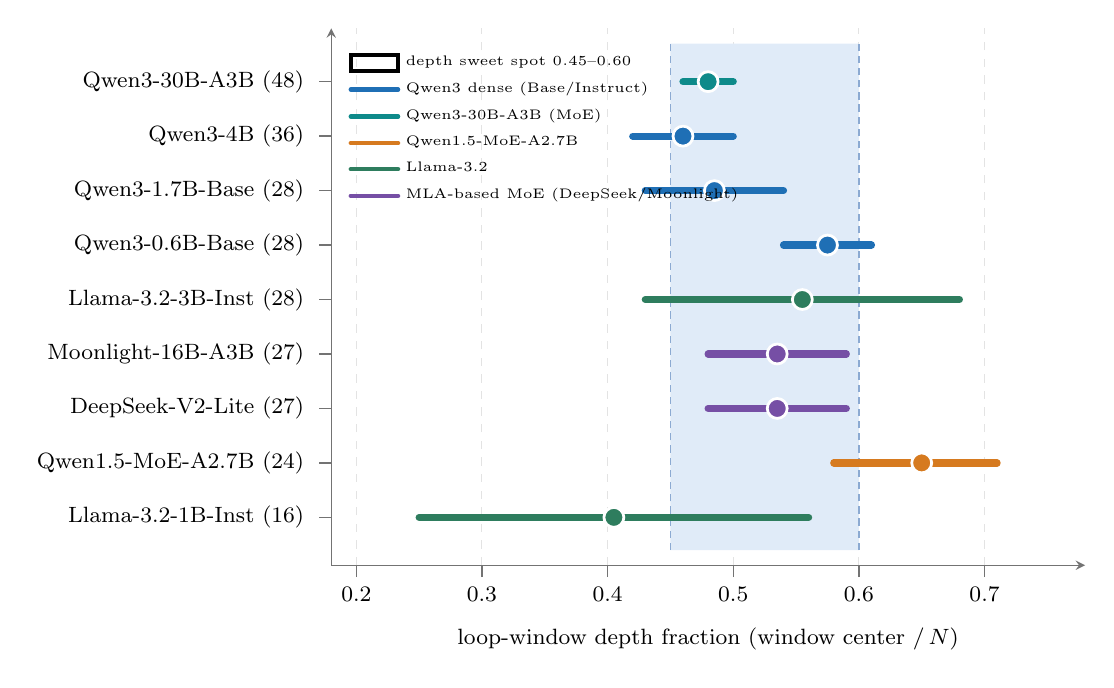
\begin{tikzpicture}
\begin{axis}[
  width=0.92\linewidth,
  height=8.4cm,
  xmin=0.18, xmax=0.78,
  ymin=-0.6, ymax=8.7,
  xtick={0.2,0.3,0.4,0.5,0.6,0.7},
  xticklabel style={font=\footnotesize},
  xlabel={\footnotesize loop-window depth fraction (window center $/\,N$)},
  xlabel style={yshift=-3pt},
  ytick={0,1,2,3,4,5,6,7,8},
  yticklabels={Llama-3.2-1B-Inst (16),
               Qwen1.5-MoE-A2.7B (24),
               DeepSeek-V2-Lite (27),
               Moonlight-16B-A3B (27),
               Llama-3.2-3B-Inst (28),
               Qwen3-0.6B-Base (28),
               Qwen3-1.7B-Base (28),
               Qwen3-4B (36),
               Qwen3-30B-A3B (48)},
  yticklabel style={font=\footnotesize, align=right, xshift=-2pt},
  axis y line=left,
  axis x line=bottom,
  axis line style={line width=0.5pt, draw=black!55},
  enlarge y limits=0.03,
  major grid style={dashed, gray!22, line width=0.35pt},
  xmajorgrids=true,
  tick align=outside,
  tick style={black!55, line width=0.5pt},
  legend style={font=\tiny, draw=none,
                at={(0.015,0.97)}, anchor=north west, fill=none,
                inner sep=2pt, row sep=0.5pt,
                fill opacity=0, text opacity=1},
  legend columns=1,
  legend cell align=left,
  legend image post style={line width=1.6pt, line cap=round},
  clip=false,
]

\addplot[fill={rgb,255:red,224;green,235;blue,248},
         draw=none, area legend]
  coordinates {(0.45,-0.6) (0.60,-0.6) (0.60,8.7) (0.45,8.7)}
  \closedcycle;
\addlegendentry{depth sweet spot $0.45$--$0.60$}

\draw[draw={rgb,255:red,140;green,170;blue,210}, line width=0.55pt,
      dash pattern=on 2.6pt off 1.8pt]
  (axis cs:0.45,-0.6) -- (axis cs:0.45,8.7);
\draw[draw={rgb,255:red,140;green,170;blue,210}, line width=0.55pt,
      dash pattern=on 2.6pt off 1.8pt]
  (axis cs:0.60,-0.6) -- (axis cs:0.60,8.7);

\addlegendimage{line width=2.4pt, line cap=round,
                color={rgb,255:red,31;green,111;blue,181}}
\addlegendentry{Qwen3 dense (Base/Instruct)}

\addlegendimage{line width=2.4pt, line cap=round,
                color={rgb,255:red,14;green,138;blue,138}}
\addlegendentry{Qwen3-30B-A3B (MoE)}

\addlegendimage{line width=2.4pt, line cap=round,
                color={rgb,255:red,214;green,122;blue,31}}
\addlegendentry{Qwen1.5-MoE-A2.7B}

\addlegendimage{line width=2.4pt, line cap=round,
                color={rgb,255:red,46;green,125;blue,94}}
\addlegendentry{Llama-3.2}

\addlegendimage{line width=2.4pt, line cap=round,
                color={rgb,255:red,118;green,79;blue,165}}
\addlegendentry{MLA-based MoE (DeepSeek/Moonlight)}

\draw[draw={rgb,255:red,46;green,125;blue,94}, line width=2.6pt,
      line cap=round] (axis cs:0.25,0) -- (axis cs:0.56,0);
\addplot[mark=*, mark size=3.6pt,
         mark options={fill={rgb,255:red,46;green,125;blue,94},
                       draw=white, line width=1.0pt},
         only marks, forget plot] coordinates {(0.405,0)};

\draw[draw={rgb,255:red,214;green,122;blue,31}, line width=2.6pt,
      line cap=round] (axis cs:0.58,1) -- (axis cs:0.71,1);
\addplot[mark=*, mark size=3.6pt,
         mark options={fill={rgb,255:red,214;green,122;blue,31},
                       draw=white, line width=1.0pt},
         only marks, forget plot] coordinates {(0.65,1)};

\draw[draw={rgb,255:red,118;green,79;blue,165}, line width=2.6pt,
      line cap=round] (axis cs:0.48,2) -- (axis cs:0.59,2);
\addplot[mark=*, mark size=3.6pt,
         mark options={fill={rgb,255:red,118;green,79;blue,165},
                       draw=white, line width=1.0pt},
         only marks, forget plot] coordinates {(0.535,2)};

\draw[draw={rgb,255:red,118;green,79;blue,165}, line width=2.6pt,
      line cap=round] (axis cs:0.48,3) -- (axis cs:0.59,3);
\addplot[mark=*, mark size=3.6pt,
         mark options={fill={rgb,255:red,118;green,79;blue,165},
                       draw=white, line width=1.0pt},
         only marks, forget plot] coordinates {(0.535,3)};

\draw[draw={rgb,255:red,46;green,125;blue,94}, line width=2.6pt,
      line cap=round] (axis cs:0.43,4) -- (axis cs:0.68,4);
\addplot[mark=*, mark size=3.6pt,
         mark options={fill={rgb,255:red,46;green,125;blue,94},
                       draw=white, line width=1.0pt},
         only marks, forget plot] coordinates {(0.555,4)};

\draw[draw={rgb,255:red,31;green,111;blue,181}, line width=2.6pt,
      line cap=round] (axis cs:0.54,5) -- (axis cs:0.61,5);
\addplot[mark=*, mark size=3.6pt,
         mark options={fill={rgb,255:red,31;green,111;blue,181},
                       draw=white, line width=1.0pt},
         only marks, forget plot] coordinates {(0.575,5)};

\draw[draw={rgb,255:red,31;green,111;blue,181}, line width=2.6pt,
      line cap=round] (axis cs:0.43,6) -- (axis cs:0.54,6);
\addplot[mark=*, mark size=3.6pt,
         mark options={fill={rgb,255:red,31;green,111;blue,181},
                       draw=white, line width=1.0pt},
         only marks, forget plot] coordinates {(0.485,6)};

\draw[draw={rgb,255:red,31;green,111;blue,181}, line width=2.6pt,
      line cap=round] (axis cs:0.42,7) -- (axis cs:0.50,7);
\addplot[mark=*, mark size=3.6pt,
         mark options={fill={rgb,255:red,31;green,111;blue,181},
                       draw=white, line width=1.0pt},
         only marks, forget plot] coordinates {(0.46,7)};

\draw[draw={rgb,255:red,14;green,138;blue,138}, line width=2.6pt,
      line cap=round] (axis cs:0.46,8) -- (axis cs:0.50,8);
\addplot[mark=*, mark size=3.6pt,
         mark options={fill={rgb,255:red,14;green,138;blue,138},
                       draw=white, line width=1.0pt},
         only marks, forget plot] coordinates {(0.48,8)};

\end{axis}
\end{tikzpicture}
\caption{\textbf{The depth-fraction rule across nine architectures.}
For each checkpoint we plot the best loop-window range $[a/N,\,b/N]$ as a horizontal bar with the window's center $(a{+}b)/(2N)$ as a filled circle. The shaded band marks the 0.45--0.60 depth fraction, which contains 7 of 9 checkpoints' optimal window centers---Qwen3 dense (0.6B--4B), Qwen3-30B-A3B MoE,DeepSeek-V2-Lite, Moonlight-16B-A3B, and Llama-3.2-3B---with only the
sub-1B distilled Llama-3.2-1B (shifted earlier) and the older Qwen1.5-MoE-A2.7B (shifted later) outside.}
\label{fig:depth-rule}
\end{figure}


